\section{Fundamentals of Hypothesis Testing}\label{S:HypTest}
%This section is under Jazz-\work\\{\scriptsize [and will evolve from face-to-face interactions with students of mathematics at Uppsala University]}.

The subset of {\bf all posable hypotheses} that remain {\bf falsifiable} is the space of {\bf scientific hypotheses}.  Roughly, a falsifiable hypothesis is one for which a statistical experiment can be designed to produce data that an experimenter can use to falsify or reject it.  In the statistical decision problem of hypothesis testing, we are interested in empirically falsifying a scientific hypothesis, i.e.~we attempt to reject an hypothesis on the basis of empirical observations or data.  Thus, hypothesis testing has its roots in the philosophy of science and is based on Karl Popper's falsifiability criterion for demarcating scientific hypotheses from the set of all posable hypotheses.

\subsection{Introduction}\label{S:HypTestIntro}
Usually, the hypothesis we attempt to reject or falsify is called the {\bf null hypothesis} or $H_0$ and its complement is called the {\bf alternative hypothesis} or $H_1$.  For example, consider the following two hypotheses:

$H_0$:  The average waiting time at an Orbiter bus stop is less than or equal to $10$ minutes.\\
$H_1$:  The average waiting time at an Orbiter bus stop is more than $10$ minutes.

If the sample mean $\overline{x}_n$ is much larger than $10$ minutes then we may be inclined to reject the null hypothesis that the average waiting time is less than or equal to $10$ minutes.  We will learn to formally test hypotheses in the sequel.

Suppose we are interested in the following hypothesis test for the bus-stop  problem:

$H_0$:  The average waiting time at an Orbiter bus stop is equal to $10$ minutes.\\
$H_1$:  The average waiting time at an Orbiter bus stop is not $10$ minutes.

Once again we can use the sample mean as the test statistic.  Our procedure for rejecting this null hypothesis is different and is often called the Wald test.

%\section{Parametric Hypothesis Testing}

More generally, suppose $X_1,X_2,\ldots,X_n \overset{IID}{\sim} F(x_1;\theta^*)$, with an unknown and fixed $\theta^* \in \BB{\Theta}$.  Let us partition the parameter space $\BB{\Theta}$ into $\BB{\Theta}_0$, the null parameter space, and $\BB{\Theta}_1$, the alternative parameter space, ie,
$$\BB{\Theta}_0 \cup \BB{\Theta}_1 = \BB{\Theta}, \qquad \text{and} \qquad \BB{\Theta}_0 \cap \BB{\Theta}_1 = \emptyset \ .$$
Then, we can formalise testing the null hypothesis versus the alternative as follows:
\[
H_0 : \theta^* \in \BB{\Theta}_0 \qquad \text{versus} \qquad H_1 :  \theta^* \subset \BB{\Theta}_1 \ .
\]
The basic idea involves finding an appropriate rejection region $\Xz_R$ within the data space $\Xz$ and rejecting $H_0$ if the observed data $x:=(x_1,x_2,\ldots,x_n)$ falls inside the rejection region $\Xz_R$,
\[
\text{If $x:=(x_1,x_2,\ldots,x_n) \in \Xz_R \subset \Xz$, then reject $H_0$, else do not reject $H_0$.} 
\]
Typically, the rejection region $\Xz_R$ is of the form:
\[
\Xz_R := \{ x:=(x_1,x_2,\ldots,x_n)  : T(x) > c \}
\]
where, $T$ is the {\bf test statistic} and $c$ is the {\bf critical value}.  Thus, the problem of finding $\Xz_R$ boils down to that of finding $T$ and $c$ that are appropriate.  Once the rejection region is defined, the possible outcomes of a hypothesis test are summarised in the following table.
\begin{table}[htbp]
\begin{center}
\caption{Outcomes of an hypothesis test.}
\begin{tabular}{c|c|c}\hline
& Do not Reject $H_0$ & Reject $H_0$ \\ \hline
$H_0$ is True & OK & Type I Error \\ \hline
$H_1$ is True & Type II Error & OK \\ \hline
\end{tabular}
\end{center}
\end{table}

\begin{definition}[Power, Size and Level of a Test]
The {\bf power function} of a test with rejection region $\Xz_R$ is
\begin{equation}\label{E:power}
\beta(\theta) := \P_{\theta}(x \in \Xz_R) \ .
\end{equation}
So $\beta(\theta)$ is the power of the test at the parameter value $\theta$, i.e.~the probability that the observed data $x$, sampled from the distribution specified by $\theta$, falls in $\Xz_R$ and thereby leads to a rejection of the null hypothesis.

The $\mathsf{size}$ of a test with rejection region $\Xz_R$ is the supreme power under the null hypothesis, i.e.~the supreme probability of rejecting the null hypothesis when the null hypothesis is true:
\begin{equation}\label{E:size}
\mathsf{size} := \sup_{\theta \in \BB{\Theta}_0} \beta(\theta) := \sup_{\theta \in \BB{\Theta}_0} \P_{\theta}(x \in \Xz_R) \ .
\end{equation}
The $\mathsf{size}$ of a test is often denoted by $\alpha$.  A test is said to have $\mathsf{level}$ $\alpha$ if its $\mathsf{size}$ is less than or equal to $\alpha$.
\end{definition}
Let us familiarize ourselves with some terminology in hypothesis testing next.
\begin{table}[htbp]
\begin{center}
\caption{Some terminology in hypothesis testing.}
\begin{tabular}{c|c|c}\hline
$\BB{\Theta}$ & Test: $H_0$ versus $H_1$ & Nomenclature \\ \hline
$\BB{\Theta} \subset \Rz^m, m \geq 1$ & $H_0: \theta^* = \theta_0$ versus $H_1: \theta^* \neq \theta_1$ & Simple Hypothesis Test \\ \hline
$\BB{\Theta} \subset \Rz^m, m \geq 1$ & $H_0: \theta^* \in \BB{\Theta}_0$ versus $H_1: \theta^* \in \BB{\Theta}_1 $ & Composite Hypothesis Test \\ \hline
$\BB{\Theta} \subset \Rz^1$ & $H_0: \theta^* = \theta_0$ versus $H_1: \theta^* \neq \theta_0$ & Two-sided Hypothesis Test \\ \hline
$\BB{\Theta} \subset \Rz^1$ & $H_0: \theta^* \geq \theta_0$ versus $H_1: \theta^* < \theta_0$ & One-sided Hypothesis Test \\ \hline
$\BB{\Theta} \subset \Rz^1$ & $H_0: \theta^* \leq \theta_0$ versus $H_1: \theta^* > \theta_0$ & One-sided Hypothesis Test \\ \hline
\end{tabular}
\end{center}
\end{table}

We introduce some widely used tests next.

\subsection{The Wald Test}\label{S:WaldTest}
The Wald test is based on a direct relationship between the $1-\alpha$ confidence interval and a $\mathsf{size}$ $\alpha$ test.  It can be used for testing simple hypotheses involving a scalar parameter.
\begin{definition}[The Wald Test]
Let $\widehat{\Theta}_n$ be an asymptotically normal estimator of the fixed and possibly unknown parameter $\theta^* \in \BB{\Theta} \subset \Rz$ in the parametric IID experiment:
\[
X_1,X_2,\ldots,X_n \overset{IID}{\sim} F(x_1;\theta^*) \enspace .
\] 
Consider testing:
\[
H_0: \theta^* = \theta_0 \qquad \text{versus} \qquad H_1: \theta^* \neq \theta_0 \enspace .
\]
Suppose that the null hypothesis is true and the estimator $\widehat{\Theta}_n$ of $\theta^*=\theta_0$ is asymptotically normal:
\[
\theta^*=\theta_0, \qquad \frac{\widehat{\Theta}_n - \theta_0}{\widehat{\mathsf{se}}_n} \rightsquigarrow \normal(0,1) \enspace .
\]
Then, the Wald test based on the test statistic $W$ is:
\[
\boxed{
\text{Reject $H_0$ when $|W|>z_{\alpha/2}$, where $W:=W((X_1,\ldots,X_n))=\frac{\widehat{\Theta}_n ((X_1,\ldots,X_n)) - \theta_0}{\widehat{\mathsf{se}}_n}$.
}
}
\]
The rejection region for the Wald test is:
\[
\boxed{
\Xz_R = \{ x:=(x_1,\ldots,x_n) : |W (x_1,\ldots,x_n) | > z_{\alpha/2} \} \enspace .
}
\]
\end{definition}
\begin{prop}[Asymptotic $\mathsf{size}$ of a Wald test]
As the sample size $n$ approaches infinity, the $\mathsf{size}$ of the Wald test approaches $\alpha$ :
\[
\boxed{
\mathsf{size} = \P_{\theta_0} \left( |W| > z_{\alpha/2} \right) \to \alpha \enspace .}
\]
\end{prop}
\begin{proof}
Let $Z \sim \normal(0,1)$.  The $\mathsf{size}$ of the Wald test, i.e.~the supreme power under $H_0$ is:
\begin{flalign*}
\mathsf{size} 
& := \sup_{\theta \in \BB{\Theta}_0} \beta(\theta) := \sup_{\theta \in \{\theta_0\}} \P_{\theta}(x \in \Xz_R) = \P_{\theta_0}(x \in \Xz_R) \\
& = \P_{\theta_0} \left( |W| > z_{\alpha/2} \right)  = \P_{\theta_0} \left( \frac{|\widehat{\theta}_n - \theta_0|}{\widehat{\mathsf{se}}_n} > z_{\alpha/2} \right) \\
& \to \P \left( |Z| > z_{\alpha/2} \right)\\
& = \alpha \enspace .
\end{flalign*}
\end{proof}
Next, let us look at the power of the Wald test when the null hypothesis is false.
\begin{prop}[Asymptotic power of a Wald test]
Suppose $\theta^* \neq \theta_0$.  The power $\beta(\theta^*)$, which is the probability of correctly rejecting the null hypothesis, is approximately equal to:
\[
\boxed{
\Phi \left( \frac{\theta_0-\theta^*}{\widehat{\mathsf{se}}_n} - z_{\alpha/2} \right) +
\left( 1- \Phi \left( \frac{\theta_0-\theta^*}{\widehat{\mathsf{se}}_n} + z_{\alpha/2} \right) \right) \enspace ,
}
\]
where, $\Phi$ is the DF of $\normal(0,1)$ RV.  Since ${\widehat{\mathsf{se}}_n} \to 0$ as $n \to 0$ the power increase with sample $\mathsf{size}$ $n$.  Also, the power increases when $|\theta_0-\theta^*|$ is large. 
\end{prop}
Now, let us make the connection between the $\mathsf{size}$ $\alpha$ Wald test and the $1-\alpha$ confidence interval explicit.
\begin{prop}[The $\mathsf{size}$ Wald test]
The $\mathsf{size}$ $\alpha$ Wald test rejects:
\[
\boxed{
\text{ $H_0: \theta^*=\theta_0$ versus $H_1: \theta^* \neq \theta_0$ if and only if $\theta_0 \notin C_n := (\widehat{\theta}_n-{\widehat{\mathsf{se}}_n} z_{\alpha/2}, \widehat{\theta}_n+{\widehat{\mathsf{se}}_n} z_{\alpha/2})$.
}}
\]
Therefore, testing the hypothesis is equivalent to verifying whether the null value $\theta_0$ is in the confidence interval.
\end{prop}
\begin{example}[Wald test for the mean waiting times at our Orbiter bus-stop]
Let us use the Wald test to attempt to reject the null hypothesis that the mean waiting time at our Orbiter bus-stop is $10$ minutes under an IID $\exponential(\lambda^*)$ model.  Let $\alpha=0.05$ for this test.  We can formulate this test as follows:
\[
H_0: \lambda^* = \lambda_0= \frac{1}{10} \quad \text{versus} \quad H_1: \lambda^* \neq \frac{1}{10}, \quad \text{where, } \quad X_1\ldots,X_{132} \overset{IID}{\sim} \exponential(\lambda^*) \enspace .
\]
Based on \hyperref[EX:ExponentialFisherInfo]{Example~\ref*{EX:ExponentialFisherInfo}} and \hyperref[LW:ExponentialMLECIOrbiter]{Labwork~\ref*{LW:ExponentialMLECIOrbiter}} we obtained the $95\%$ confidence interval to be $[0.0914, 0.1290]$. Since our null value $\lambda_0=0.1$ belongs to this confidence interval, we fail to reject the null hypothesis from a $\mathsf{size}$ $\alpha=0.05$ Wald test.
\end{example}

We can use bootstrap-based confidence interval $C_n$ in conjunction with Wald test as shown by the next example.

\begin{example}[Wald test of the bootstrapped correlation coefficient]
Recall the problem of estimating the confidence interval for the correlation coefficient between the LSAT scores ($Y_1,\ldots,Y_{15}$) and the GPA ($Z_1,\ldots,Z_{15}$) in \hyperref[LW:LSATGPACorrBoot]{Labwork~\ref*{LW:LSATGPACorrBoot}}.  We assumed that the bivariate data $(Y_i,Z_i) \overset{IID}{\sim} F^*$, such that $F^* \in \{ \text{all bivariate DFs} \}$. Suppose we are interested in testing the null hypothesis that the true correlation coefficient $\theta^*$ is $0$:
\[
H_0: \theta^* = \theta_0 = 0 \quad \text{versus} \quad H_1: \theta^* \neq 0, \quad \text{where} \quad  \theta^* = \frac{\int \int (y-\E(Y))(z-\E(Z))dF(y,z)}{\sqrt{\int (y-\E(Y))^2 dF(y) \int (z-\E(Z))^2 dF(z)}} \enspace .
\]
Since the percentile-based $95\%$ bootstrap confidence interval for the plug-in estimate of the correlation coefficient from \hyperref[LW:LSATGPACorrBoot]{Labwork~\ref*{LW:LSATGPACorrBoot}} was $[0.2346, 0.9296]$ and this interval does not contain $0$, we can reject the null hypothesis that the correlation coefficient is $0$ using a $\mathsf{size}$ $\alpha=0.05$ Wald test.
\end{example}

\subsection{A Composite Hypothesis Test}
Often, we are interested in a testing a composite hypothesis, i.e.~one in which  the null hypothesis is not a singleton set.  We revisit the Orbiter waiting time problem from this perspective next.
\begin{figure}[htpb]
\caption{Plot of power function $\beta(\lambda)$ for different values of the critical value $c$ and the $\mathsf{size}$ $\alpha$ as function of the critical values.
\label{F:ExponentialTestOrbiter}}
\centering   \makebox{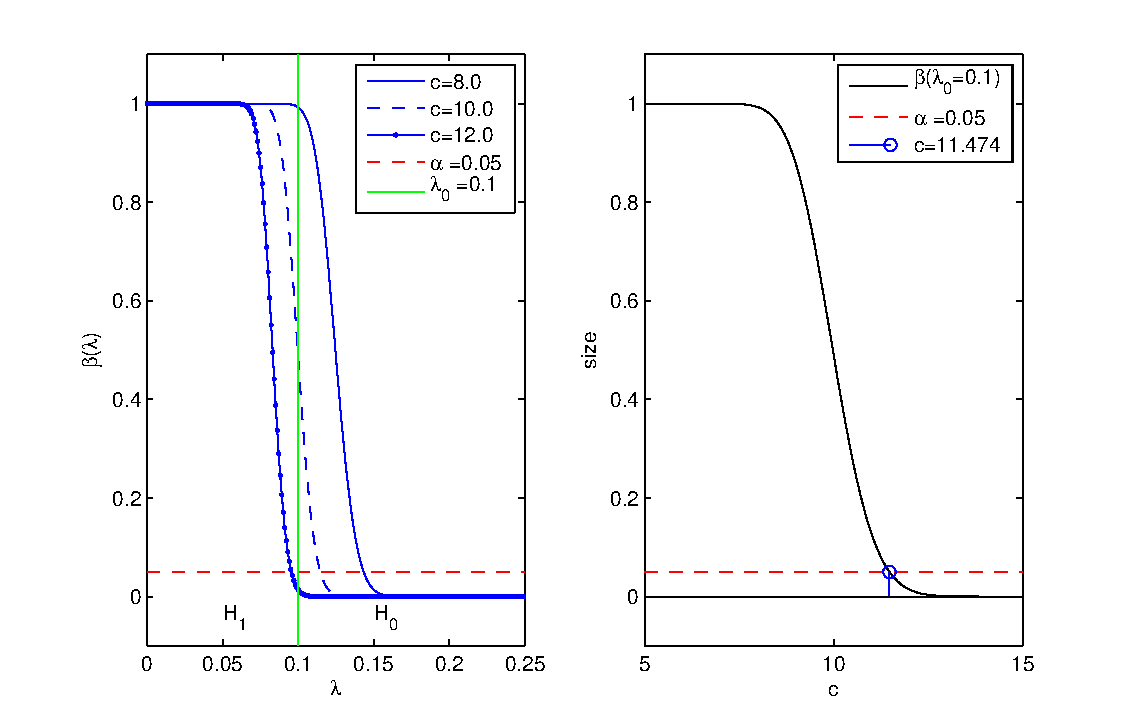
\includegraphics[width=6.5in]{figures/ExponentialTestOrbiter}}
\end{figure}

\begin{example}[Testing the Mean Waiting Time at an Orbiter Bus-stop]
Let us test the following null hypothesis $H_0$.

$H_0$:  The average waiting time at an Orbiter bus stop is less than or equal to $10$ minutes.\\
$H_1$:  The average waiting time at an Orbiter bus stop is more than $10$ minutes.

We have observations of $n=132$ waiting times $x_1,x_2,\ldots,x_{132}$ at the Orbter bus-stop with $\overline{x}_{132}=9.0758$.  Let us assume a parametric model, say,
\[
X_1,X_2,\ldots,X_n \overset{IID}{\sim} \exponential(\lambda^*)
\]
with an unknown and fixed $\lambda^* \in \BB{\Lambda}=(0,\infty)$.  Since the parameter $\lambda$ of an $\exponential(\lambda)$ RV is the reciprocal of the mean waiting time, we can formalise the above hypothesis testing problem of $H_0$ versus $H_1$ as follows:
\[
H_0 : \lambda^* \in \BB{\Lambda}_0 = [1/10,\infty) \qquad \text{versus} \qquad H_1 :  \lambda^* \in \BB{\Lambda}_1 = (0,1/10) 
\]
Consider the test:
\[
\text{Reject $H_0$ if $T>c$.}
\] 
where the test statistic $T=\overline{X}_n$ and the rejection region is:
\[
\Xz_R = \{ (x_1,x_2,\ldots,x_n) : T(x_1,x_2,\ldots,x_n) > c \} \enspace .
\]
Since the sum of $n$ IID $\exponential(\lambda)$ RVs is $\gammA(\lambda,n)$ distributed, the power function is:
\begin{flalign*}
\beta(\lambda) &= \P_{\lambda} \left(\overline{X}_n > c \right) = \P_{\lambda}\left(\sum_{i=1}^n{X_i} > nc \right) = 1- \P_{\lambda}\left(\sum_{i=1}^n{X_i} \leq nc \right)\\
&= 1 - F\left( nc; \lambda, n \right) 
= 1- \frac{1}{\Gamma(n)}\int_0^{\lambda n c} y^{n-1} \exp(-y) dy \\
&= 1- {\tt gammainc}(\lambda n c, n)
\end{flalign*}
Clearly, $\beta(\lambda)$ is a decreasing function of $\lambda$ as shown in \hyperref[F:ExponentialMLECIOrbiter]{Figure~\ref*{F:ExponentialTestOrbiter}}.  Hence the $\mathsf{size}$ of the test as a function of the critical region specified by the critical value $c$ is:
\begin{flalign*}
\mathsf{size} 
&= \sup_{\lambda \in \BB{\Lambda}_0} \beta(\lambda)
= \sup_{\lambda \geq 1/10} \beta(\lambda)=\beta(1/10)=1- {\tt gammainc}(132 c/10, 132)
\end{flalign*}
For a $\mathsf{size}$ $\alpha=0.05$ test we numerically solve for the critical value $c$ that satisfies: $$0.05=1- {\tt gammainc}(132 c/10, 132)$$ by trial and error as follows:
\begin{VrbM}
>> lambda0=1/10
lambda0 =    0.1000
>> S=@(C)(1-gammainc(lambda0*n*C,n)); % size as a function of c
>> Cs=[10 11 11.474 12 13] % some critical values c
Cs =   10.0000   11.0000   11.4740   12.0000   13.0000
>> Size=arrayfun(S,Cs) % corresponding size
Size =    0.4884    0.1268    0.0499    0.0143    0.0007
\end{VrbM}  
Thus, we reject $H_0$ when $\overline{X}_n>11.4740$ for a level $\alpha=0.05$ test.  Since our observed test statistic $\overline{x}_{132}=9.0758 < 11.4740$ we fail to reject the null hypothesis that the mean waiting time is less than or equal to $10$ minutes.  Therefore, there is no evidence that the Orbiter bus company is violating its promise of an average waiting time of no more than $10$ minutes.
\end{example}



\subsection{p-values}\label{S:p-values}
It is desirable to have a more informative decision than simply reporting "reject $H_0$'' or ``fail to reject $H_0$.''  For instance, we could ask whether the test rejects $H_0$ for each $\mathsf{size}=\alpha$.  Typically, if the test rejects at $\mathsf{size}$ $\alpha$ it will also reject at a larger $\mathsf{size}$ $\alpha' > \alpha$.  Therefore, there is a smallest $\mathsf{size}$ $\alpha$ at which the test rejects $H_0$ and we call this $\alpha$ the $\pvalue$ of the test.

\begin{figure}[h]
\caption{The smallest $\alpha$ at which a $\mathsf{size}$ $\alpha$ test rejects the null hypothesis $H_0$ is the $\pvalue$.}\label{F:pvalue}
\begin{center}
\fbox{
\setlength{\unitlength}{1mm}
\begin{picture}(130,50)(0,-2)
\thicklines
\put(10,30){\fbox{Reject $H_0$?~}}
\put(30,10){{No~}}
\put(30,40){{Yes~}}

\put(40,5){\vector(0,1){40}}
\put(40,5){\vector(1,0){70}}
\put(59,4){$\bullet$}
\put(70,15){\vector(-1,-1){10}}
\put(70,15){$\pvalue$}

\put(40,1){$0$}
\put(90,1){$1$}
\put(65,-1){$\mathsf{size}$}

\put(40,10){\line(1,0){20}}
\put(60,10){\line(0,1){30}}
\put(60,40){\line(1,0){30}}

\end{picture}
}
\end{center}
\end{figure}

\begin{definition}[p-value]
Suppose that for every $\alpha \in (0,1)$ we have a $\mathsf{size}$ $\alpha$ test with rejection region $\Xz_{R,\alpha}$ and test statistic $T$.  Then,
\[
\pvalue := \inf \{ \alpha: T(X) \in \Xz_{R,\alpha} \} \enspace .
\]
That is, the $\pvalue$ is the smallest $\alpha$ at which a $\mathsf{size}$ $\alpha$ test rejects the null hypothesis.
\end{definition}

If the evidence against $H_0$ is strong then the $\pvalue$ will be small.  However, a large $\pvalue$ is not strong evidence in favour of $H_0$.  This is because a large $\pvalue$ can occur for two reasons:
\begin{enumerate}
\item $H_0$ is true.
\item $H_0$ is false but the test has low power.
\end{enumerate}
Finally, it is important to realise that $\pvalue$ is not the probability that the null hypothesis is true, i.e.~$\pvalue \neq \P(H_0|x)$, where $x$ is the data.  The following tabulation of evidence scale is useful.
\begin{table}
\caption{Evidence scale against the null hypothesis in terms of the range of $\pvalue$.}\label{T:pvalueEvidenceScale}
\begin{center}
\begin{tabular}{|c|c|}
\hline
$\pvalue$ range & Evidence \\ \hline
$(0, 0.01]$ & very strong evidence against $H_0$\\
$(0.01, 0.05]$ & strong evidence against $H_0$\\
$(0.05, 0.1]$ & weak evidence against $H_0$\\
$(0.1,1)$ & little or no evidence against $H_0$\\
\hline
\end{tabular}
\end{center} 
\end{table}
The next proposition gives a convenient expression for the $\pvalue$ for certain tests.
\begin{prop}[The $\pvalue$ of a hypothesis test]
Suppose that the $\mathsf{size}$ $\alpha$ test based on the test statistic $T$ and critical value $c_{\alpha}$ is of the form:
\[
\text{Reject $H_0$ if and only if $T:=T((X_1,\ldots,X_n))> c_{\alpha}$,}
\]
then
\[
\pvalue = \sup_{\theta \in \BB{\Theta}_0} \P_{\theta}(T((X_1,\ldots,X_n)) \geq t:=T((x_1,\ldots,x_n))) \enspace ,
\]
where, $(x_1,\ldots,x_n)$ is the observed data and $t$ is the observed value of the test statistic $T$.  In words, the $\pvalue$ is the supreme probability under $H_0$ of observing a value of the test statistic the same as or more extreme than what was actually observed.
\end{prop}
Let us revisit the Orbiter waiting times example from the $\pvalue$ perspective.
\begin{example}[$\pvalue$ for the parametric Orbiter experiment]
Let the waiting times at our bus-stop be $X_1,X_2,\ldots,X_{132} \overset{IID}{\sim} \exponential(\lambda^*)$.  Consider the following testing problem:
\[
H_0: \lambda^*=\lambda_0=\frac{1}{10} \quad \text{versus} \quad H_1: \lambda^* \neq \lambda_0 \enspace .
\]
We already saw that the Wald test statistic is:
\[
W:=W(X_1,\ldots,X_n)= \frac{\widehat{\Lambda}_n-\lambda_0}{\widehat{\mathsf{se}}_n(\widehat{\Lambda}_n)} = \frac{\frac{1}{\overline{X}_n}-\lambda_0}{\frac{1}{\sqrt{n}\overline{X}_n}} \enspace .
\]
The observed test statistic is:
\[
w=W(x_1,\ldots,x_{132})=
\frac{\frac{1}{\overline{X}_{132}}-\lambda_0}{\frac{1}{\sqrt{132}\overline{X}_{132}}}
= \frac{\frac{1}{9.0758}-\frac{1}{10}}{\frac{1}{\sqrt{132} \times 9.0758}} = 1.0618 \enspace .
\]
Since, $W \rightsquigarrow Z \sim \normal(0,1)$, the $\pvalue$ for this Wald test is:
\begin{flalign*}
\pvalue 
&= \sup_{\lambda \in \BB{\Lambda}_0} \P_{\lambda} (|W|>|w|)= \sup_{\lambda \in \{\lambda_0\}} \P_{\lambda} (|W|>|w|) =  \P_{\lambda_0} (|W|>|w|) \\
& \to \P (|Z|>|w|)=2 \Phi(-|w|)=2 \Phi(-|1.0618|)=2 \times 0.1442=0.2884 \enspace .
\end{flalign*}
Therefore, there is little or no evidence against $H_0$ that the mean waiting time under an IID $\exponential$ model of inter-arrival times is exactly ten minutes.
\end{example}
%\section{Parametric Bootstrap-based Test}

\subsection{Permutation Test for the equality of any two DFs}\label{S:PermTest}

Permutation test is a non-parametric exact method for testing whether two distributions are the same.  It is non-parametric because we do not impose any restrictions on the class of DFs that the unknown DF should belong to.  It is exact because we do not have any asymptotic approximations involving sample size approaching infinity.  So this test works for any sample size.

Formally, we suppose that:
\[
X_1,X_2,\ldots,X_m \overset{IID}{\sim} F^* \quad \text{and} \quad X_{m+1}, X_{m+2},\ldots,X_{m+n} \overset{IID}{\sim} G^* \enspace ,
\]
are two sets of independent samples.  The possibly unknown DFs $F^*,G^* \in \{ \text{all DFs} \}$.  Now, consider the following hypothesis test:
\[
H_0: F^*=G^* \quad \text{versus} \quad H_1: F^* \neq G^* \enspace .
\]
Let our test statistic $T(X_1,\ldots,X_m,X_{m+1},\ldots,X_{m+n})$ be some sensible one -- $T$ is large when $F^*$ is too different from $G^*$, say:
\[
T:=T(X_1,\ldots,X_m,X_{m+1},\ldots,X_{m+n})= \abs \left( \frac{1}{m} \sum_{i=1}^m X_i -  \frac{1}{n} \sum_{i=m+1}^n X_i  \right) \enspace .
\]
Then the idea of a permutation test is as follows:
\begin{enumerate}
\item Let $N:=m+n$ be the pooled sample size and consider all $N!$ permutations of the observed data $x_{\mathsf{obs}}:=(x_1,x_2,\ldots,x_m,x_{m+1},x_{m+2},\ldots,x_{m+n})$.
\item For each permutation of the data compute the statistic $T(\text{permuted data $x$})$ and denote these $N!$ values of $T$ by $t_1,t_2,\ldots,t_{N!}$.
\item Under $H_0: X_1,\ldots,X_m,X_{m+1},\ldots,X_{m+n} \overset{IID}{\sim}F^*=G^*$, each of the permutations of $x= (x_1,x_2,\ldots,x_m,x_{m+1},x_{m+2},\ldots,x_{m+n})$ has the same joint probability $\prod_{i=1}^{m+n} f(x_i)$, where $f(x_i)=dF(x_i)=dG(x_i)$.  Therefore, the transformation of the data by our statistic $T$ also has the same probability over the values of $T$, namely $\{t_1,t_2,\ldots,t_{N!}\}$.  Let $\P_0$ be this permutation distribution that is dicrete and uniform over  $\{t_1,t_2,\ldots,t_{N!}\}$.
\item Let $t_{\mathsf{obs}} := T(x_{\mathsf{obs}})$ be the observed value of the statistic.
\item Assuming we reject $H_0$ when $T$ is large, the $\pvalue$ is:
\[
\pvalue = \P_0 \left( T \geq t_{\mathsf{obs}} \right) = \frac{1}{N!} \left( \sum_{j=1}^{N!} \BB{1} (t_j  \geq t_{\mathsf{obs}}) \right), \qquad  \BB{1} (t_j \geq t_{\mathsf{obs}}) =
\begin{cases}
1 & \text{if } \quad t_j \geq t_{\mathsf{obs}} \\
0 & \text{otherwise} 
\end{cases}
\]
\end{enumerate}

Let us look at a small example involving the diameters of coarse venus shells ({\em Dosinia anus}) that Guo Yaozong and Chen Shun found on the left and right sides of the New Brighton prier in Spring 2007.  We are interested in testing the hypothesis that the distribution of shell diameters for this bivalve species is the same on both sides of the pier.  
\begin{example}[Guo-Chen Experiment with Venus Shell Diameters]
Let us look at the first two samples $x_1$ and $x_2$ from the left of pier and the first sample from the right side of pier, namely $x_3$.  Since the permutation test is exact, we can use this small data set with merely three samples to conduct the following hypothesis test:
\[
H_0: X_1,X_2,X_3 \overset{IID}{\sim} F^*=G^*, \qquad H_1: X_1,X_2 \overset{IID}{\sim} F^*, X_3 \overset{IID}{\sim} G^*, \quad F^* \neq G^* \enspace .
\] 
Let us use the test statistic:
\[
T(X_1,X_2,X_3)=\abs \left( \frac{1}{2} \sum_{i=1}^2 X_i -  \frac{1}{1} \sum_{i=2+1}^3 X_i  \right)=\abs \left( \frac{X_1+x_2}{2} -  \frac{X_3}{1} \right) \enspace .
\]
The data giving the shell diameters in millimetres and $t_{\mathsf{obs}}$ are:
\[
(x_1,x_2,x_3) = (52,54,58) \quad \text{and} \quad t_{\mathsf{obs}}=\abs \left( \frac{52+54}{2} - \frac{58}{1} \right) = \abs (53-58) = \abs(-5)=5 \enspace .
\]
Let us tabulate the $(2+1)!=3!=3\times2\times1=6$ permutations of the data $(x_1,x_2,x_3) = (52,54,58)$, the corresponding values of $T$ and their probabilities under the null hypothesis, i.e., the permutation distribution $\P_0(T)$.
\begin{center}
\begin{tabular}{c c c}
\hline
Permutation & $t$ & $\P_0(T=t)$ \\ \hline
$(52,54,58)$ & $5$ & $\frac{1}{6}$ \\
$(54,52,58)$ & $5$ & $\frac{1}{6}$  \\
$(52,58,54)$ & $1$ & $\frac{1}{6}$  \\
$(58,52,54)$ & $1$ &$\frac{1}{6}$  \\
$(58,54,52)$ & $4$ & $\frac{1}{6}$  \\
$(54,58,52)$ & $4$ & $\frac{1}{6}$  \\ \hline
\end{tabular}
\end{center}
From the table, we get:
\[
\pvalue = \P_0 \left( T \geq t_{\mathsf{obs}}\right) =  \P_0 \left( T \geq 5 \right) = \frac{1}{6}+ \frac{1}{6}= \frac{2}{6}= \frac{1}{3} \approxeq 0.333 \enspace . 
\]
Therefore, there is little to no evidence against $H_0$.
\end{example}

When the pooled sample size $N=m+n$ gets large, $N!$ would be too numerous to tabulate exhaustively.  In this situation, we can use a Monte Carlo approximation of the $\pvalue$ by generating a large number of random permutations of the data according to the following Steps:

\begin{enumerate}
\item[\sf{Step 1}:] Compute the observed statistic $t_{\mathsf{obs}} := T(x_{\mathsf{obs}})$ of data $x_{\mathsf{obs}}:=(x_1,\ldots,x_m,x_{m+1},\ldots,x_{m+n})$.
\item[\sf{Step 2}:] Randomly permute the data and compute the statistic again from the permuted data.
\item[\sf{Step 3}:] Repeat {\sf Step 2} $B$ times and let $t_1,\ldots,t_B$ denote the resulting values ($B$ is large, say $1000$).
\item[\sf{Step 4}:] The (Monte Carlo) approximate $\pvalue$ is:
\[
\frac{1}{B} \sum_{j=1}^B \BB{1}(t_j \geq t_{\mathsf{obs}} ) \enspace .
\]
\end{enumerate}
Next we implement the above algorithm on the full data set of Guo and Chen obtained from coarse venus shells sampled from the two sides of the New Brighton pier. 
\begin{labwork}[Approximate $\pvalue$ of a permutation test of shell diameters]\label{LW:Shells}
Test the null hypothesis that the distribution of the diameters of coarse venus shells are the same on both sides of the New Brighton pier. 
\VrbMf[label=Shells.m]{scripts/Shells.m}
When we execute the script to perform a permutation test and approximate the $\pvalue$, we obtain:
\begin{VrbM}
>> Shells
ApproxPValue =    0.8576
\end{VrbM}
Therefore, there is little or no evidence against the null hypothesis.
\end{labwork}

\subsection{Pearson's Chi-Square Test for Multinomial Trials}\label{S:Chi2}

We derive the $\chisquare$ distribution introduced by Karl Pearson in 1900 [{\em Philosophical Magazine}, Series 5, {\bf 50}, 157-175].  This historical work laid the foundations of modern statistics by showing why an experimenter cannot simply plot experimental data and just assert the correctness of his or her hypothesis.  This derivation is adapted from Donald E.~Knuth's treatment [{\em Art of Computer Programming, Vol.~II, Seminumerical Algorithms}, 3rd Ed., 1997, pp.~55-56].  We show how $\demoivre$, $\multinomial$, $\poisson$ and the $\normal$ random vectors conspire to creare the $\chisquare$ random variable.

{\em Part 1: \demoivre~trials}\\
Consider $n$ independent and identically distributed $\demoivre (\theta_1,\ldots,\theta_k)$ random vectors (\rv s):
\[
X_1,X_2,\ldots,X_n \overset{IID}{\sim} \demoivre (\theta_1,\ldots,\theta_k) \enspace .
\]
Recall from \hyperref[M:deMoivreRVec]{Model~\ref*{M:deMoivreRVec}} that $X_1 \sim \demoivre (\theta_1,\ldots,\theta_k)$ means $\P(X_1=e_i)=\theta_i$ for $i\in\{1,\ldots,k\}$, where $e_1,\ldots,e_k$ are ortho-normal basis vectors in $\Rz^k$. 
Thus, for each $i \in \{1,2,\ldots,n\}$, the corresponding  $X_i$ has $k$ components, i.e.~$X_i:=(X_{i,1},X_{i,2},\ldots,X_{i,k})$.

{\em Part 2: \multinomial~trial}\\
Suppose we are only interested in the experiment induced by their sum:
\[
Y := (Y_1,\ldots,Y_k) := \sum_{i=1}^n X_i :=  \sum_{i=1}^n (X_{i,1},X_{i,2},\ldots,X_{i,k}) = \left( \sum_{i=1}^n X_{i,1}, \sum_{i=1}^n X_{i,2},\ldots, \sum_{i=1}^n X_{i,k} \right) \enspace .
\]
The \rv~$Y$, being the sum of $n$ IID $\demoivre(\theta_1,\ldots,\theta_k)$ \rv s, is the $\multinomial(n,\theta_1,\ldots,\theta_k)$ \rv~of  \hyperref[M:Multinomial]{Model~\ref*{M:Multinomial}} and the probability that $Y:=(Y_1,\ldots,Y_k) = y := (y_1,\ldots,y_k)$ is:
\[
 \frac{n!}{y_1! y_2! \cdots y_k!} \prod_{i=1}^k \theta_i^{y_i} \enspace .
\]
The support of the \rv~$Y$, i.e.~the set of possible realisations of $y:= (y_1,\ldots,y_k)$ is:
\[
\Yz := \{ (y_1,\ldots,y_k) \in \Zz_+^k : \sum_{i=1}^k y_i = n \} \enspace .
\]
{\em Part 3: Conditional sum of \poisson~trials}\\
Here we consider an alternative formulation of the $\multinomial(n,\theta_1,\ldots,\theta_k)$ \rv~$Y$.  Suppose,
\[
Y_1 \sim \poisson(n \theta_1), Y_2 \sim \poisson(n \theta_2), \ldots, Y_k \sim \poisson(n \theta_k) \enspace ,
\]
and that $Y_1,\ldots,Y_k$ are independent.  Recall from \hyperref[M:Poisson]{Model~\ref*{M:Poisson}} that $Y_i \sim \poisson(n\theta_i)$ means $\P(Y_i=y_i)=e^{-n\theta_i} (n\theta_i)^{y_i}/y_i!$ for $y_i \in \{0,1,\ldots\}$.  Then, the joint probability probability of the \rv~$(Y_1,\ldots,Y_k)$ is the product of the independent $\poisson$ probabilities:
\begin{flalign*}
\P\left( (Y_1,\ldots,Y_k) = (y_1,\ldots,y_k) \right) 
&:= \P \left( Y_1=y_1,\ldots,Y_k=y_k \right) 
= \prod_{i=1}^k \P(Y_i=y_i) = \prod_{i=1}^k{ \frac{e^{-n\theta_i} (n\theta_i)^{y_i}}{y_i!} } \\
& 
= \frac{ \prod_{i=1}^k e^{-n\theta_i} n^{y_i} \theta_i^{y_i}}{ \prod_{i=1}^k{ y_i!} }
=\left(e^{-n \sum_{i=1}^k \theta_i} n^{\sum_{i=1}^k y_i} \prod_{i=1}^k \theta_i^{y_i}\right) \frac{1}{ \prod_{i=1}^k{ y_i!} } \\
& =  \frac{  e^{-n} n^{n} \prod_{i=1}^k \theta_i^{y_i}}{ \prod_{i=1}^k{ y_i!} }
\enspace .
\end{flalign*}
Now, the probability that sum $Y_1+\cdots+Y_k$ will equal $n$ is obtained by summing over the probabilities of all $(y_1,\ldots,y_k) \in \Yz$:
\begin{flalign*}
\P\left(\sum_{i=1}^k Y_i = n \right)
& = \sum_{\substack{(y_1,\ldots,y_k)\\ \in\Yz}}  \P\left( (Y_1,\ldots,Y_k) = (y_1,\ldots,y_k) \right) =  \sum_{\substack{(y_1,\ldots,y_k)\\ \in\Yz}}  \frac{  e^{-n} n^{n} \prod_{i=1}^k \theta_i^{y_i}}{ \prod_{i=1}^k{ y_i!} } \\
& = e^{-n} n^{n} \frac{1}{n!} 
\underset {=\P(\Yz)=1}{\underbrace{\left( \sum_{\substack{(y_1,\ldots,y_k)\\ \in\Yz}}   \frac{n!}{ \prod_{i=1}^k{ y_i!} } \prod_{i=1}^k \theta_i^{y_i} \right)}} = \frac{e^{-n} n^{n}}{n!}
\enspace .
\end{flalign*}
Finally, the conditional probability that $(Y_1,\ldots,Y_k)=(y_1,\ldots,y_k)$ given $\sum_{i=1}^k Y_i = n$ is:
\begin{multline*}
\P \left( (Y_1,\ldots,Y_k)=(y_1,\ldots,y_k) \vert \sum_{i=1}^k Y_i = n \right) = 
\frac{\P \left( (Y_1,\ldots,Y_k)=(y_1,\ldots,y_k) , \sum_{i=1}^k Y_i = n \right)}{\P \left( \sum_{i=1}^k Y_i = n \right) } \\
= \frac{\P \left( (Y_1,\ldots,Y_k)=(y_1,\ldots,y_k) \right)}{\P \left( \sum_{i=1}^k Y_i = n \right) } 
= \frac{  e^{-n} n^{n} \prod_{i=1}^k \theta_i^{y_i}}{ \prod_{i=1}^k{ y_i!} } \frac{n!} {e^{-n} n^{n}} =  \frac{n!}{y_1! y_2! \cdots y_k!} \prod_{i=1}^k \theta_i^{y_i} \enspace .
\end{multline*}
Therefore, we may also think of the random vector $Y:=(Y_1,\ldots,Y_k) \sim \multinomial(n,\theta_1,\ldots,\theta_k)$ as $k$ independent $\poisson$ random variables, $Y_1 \sim \poisson(n \theta_1), \ldots, Y_k \sim \poisson(n \theta_k)$, that have been conditioned on their sum $\sum_{i=1}^nY_i$ being $n$.

{\em Part 4: The $\normal$ approximation of the centred and scaled $\poisson$}\\
Recall from \hyperref[M:Poisson]{Model~\ref*{M:Poisson}} that the expectation and variance of a RV $Y_i \sim \poisson(n\theta_i)$ are $\E(Y_i)=\V(Y_i)=n\theta_i$.  Let $Z_i$ be $\E(Y_i)$-centred and $\sqrt{\V(Y_i)}$-scaled $Y_i$ and \[
Z_i :=  \frac{Y_i - \E(Y_i)}{\sqrt{\V(Y_i)}} = \frac{Y_i - n \theta_i}{\sqrt{n \theta_i}} \enspace .
\]
The condition that $Y_1+\cdots+Y_k=n$ is equivalent to requiring that $\sqrt{\theta_1} Z_1 +\cdots+\sqrt{\theta_k} Z_k = 0$, since:
\begin{multline*}
\sum_{i=1}^k {Y_i} =n 
\iff \sum_{i=1}^k {Y_i} -n = 0
\iff \sum_{i=1}^k {Y_i} - n \sum_{i=1}^k {\theta_i} = 0
\iff \sum_{i=1}^k {Y_i - n \theta_i} = 0 \\
\iff \sum_{i=1}^k  \frac{Y_i - n \theta_i}{\sqrt{n }} = 0
\iff \sum_{i=1}^k \sqrt{\theta_i} \frac{Y_i - n \theta_i}{\sqrt{n \theta_i}} = 0
\iff \sum_{i=1}^k \sqrt{\theta_i} Z_i = 0 \enspace .
\end{multline*}
Now consider the support of the \rv~$Z:=(Z_1,\ldots,Z_k)$ conditioned on $\sum_{i=1}^k \sqrt{\theta_i} Z_i = 0$, i.e.~the hyper-plane of $(k-1)$-dimensional vectors:
\[
\Hz := \{ (z_1,\ldots,z_k) : \sqrt{\theta_1} z_1 +\cdots+\sqrt{\theta_k} z_k = 0 \} 
\]
Each $Z_i \rightsquigarrow \normal(0,1)$ by the central limit theorem.  Therefore, for large values of $n$, each $Z_i$ is approximately distributed as the $\normal(0,1)$ RV with PDF $f(z_i;0,1)=(2\pi)^{-1/2}\exp(-z_i^2/2)$.  Since the $Z_i$s are independent except for the condition that they lie in $\Hz$, the point in a differential volume $dz_2\ldots dz_k$ of $\Hz$ occur with probability approximately proportional to:
 \[
 \exp(-z_1^2/2) \times \cdots \times \exp(-z_k^2/2)  = \exp(-(z_1^2+\cdots+z_k^2)/2)
 \]

{\em Part 5: $\chisquare$ distribution as the sum of squared $\normal$s}\\
We are interested in the sum of the area of squares with side-lengths $Z_1,\ldots,Z_k$.  Let $V$ be the desired sum of squares:
\[
\qquad V := \sum_{i=1}^k Z_i^2 =  \sum_{i=1}^k \frac{\left(Y_i - n \theta_i \right)^2}{{n \theta_i}}  , \quad \text{such that} \quad Z_i \rightsquigarrow \normal(0,1), \quad \sum_{i=1}^k \sqrt{\theta_i} Z_i = 0 \enspace .
\]
The probability that $V \leq v$ as $n \to \infty$ is:
\[
\frac{\int_{\substack{(z_1,\ldots,z_k) \in \Hz \ \text{and} \ \sum_{i=1}^k{z_i^2} \leq v}} \exp(-(z_1^2+\cdots+z_k^2)/2) \ dz_2\ldots dz_k} {\int_{\substack{(z_1,\ldots,z_k) \in \Hz}} \exp(-(z_1^2+\cdots+z_k^2)/2) \ dz_2\ldots dz_k}
\]
Since the $(k-1)$-dimensional hyper-plane $\Hz$ passes through the origin of  $\Rz^k$, the domain of integration in the numerator above is the interior of a $(k-1)$-dimensional hyper-sphere of radius $\sqrt{v}$ that is centred at the origin.  Using a transformation of the above ratio of integrals into generalised polar co-ordinates with radius $\chi$  and angles $\alpha_1,\ldots,\alpha_{k-2}$, we get:
\[
\frac{\int_{\chi^2\leq v} \exp(-\chi^2/2) \chi^{k-2} g(\alpha_1,\ldots,\alpha_{k-2}) d \chi d \alpha_1\cdots d \alpha_{k-2}} {\int \exp(-\chi^2/2) \chi^{k-2} g(\alpha_1,\ldots,\alpha_{k-2}) d \chi d \alpha_1\cdots d \alpha_{k-2}} \enspace ,
\]
for some function $g$ of the angles [See Problem 15 in {\em Art of Computer Programming, Vol.~II, Seminumerical Algorithms}, 3rd Ed., 1997, pp.~59].   The integration over the $(k-2)$ angles results in the same factor that cancels between the numerator and the denominator.  This yields the formula for the probability that $V \leq v$ as $n \rightarrow \infty$:
\[
\lim_{n \to \infty} \P(V \leq v) =  \frac{\int_0^{\sqrt{v}}\exp(-\chi^2/2) \chi^{k-2} d \chi} {\int_0^{\infty}\exp(-\chi^2/2) \chi^{k-2} \ d \chi} \enspace .
\]  
By substituting $t=\chi^2/2$, we can express the integrals in terms of the incomplete Gamma function defined as $\gamma(a,x) :=  \int_0^{a} \exp(-t) t^{a-1} \ dt$ as follows:
\[
\P(V \leq v) = \gamma \left( \frac{k-1}{2},\frac{v}{2} \right) / \Gamma \left(\frac{k-1}{2} \right) \enspace .
\]
This is the DF of the $\chisquare$ distribution with $k-1$ degrees of freedom.

\begin{model}[$\chisquare(k)$ RV]  Given a parameter $k \in \Nz$ called degrees of freedom, we say that $V$ is a $\chisquare(k)$ RV if its PDF is:
\[
f(v; k) :=  \frac{v^{(k/2)-1}e^{-v/2}}{2^{k/2}\Gamma(k/2)} \BB{1}_{\{v \in \Rz: v>0\}}(v)
\]
Also, $\E(V)=k$ and $\V(V) = 2k$.
\end{model}

We can use the test statistic: 
$$T:= T(Y_1,\ldots,Y_k) = \frac{\left(Y_1 - n \theta^*_1 \right)^2}{n \theta^*_1}+\cdots+\frac{\left(Y_k - n \theta^*_k \right)^2}{n \theta^*_k}$$
to test the null hypothesis $H_0$ that may be formalised in three equivalent ways:
\begin{flalign*}
& H_0: X_1,X_2,\ldots,X_n \overset{IID}{\sim} \demoivre(\theta_1^*,\ldots,\theta_k^*)~\rv \\
\iff 
& H_0:
Y:= (Y_1,\ldots,Y_k) = \sum_{i=1}^n X_i \sim \multinomial(n,\theta_1^*,\ldots,\theta_k^*)~\rv \\
\iff 
& H_0:
Y_1 \overset{IND}{\sim} \poisson(n\theta_1)~\mbox{RV},\ldots,Y_k \overset{IND}{\sim} \poisson(n\theta_k)~\mbox{RV} \ \text{given that} \ \sum_{i=1}^k Y_i = n
\end{flalign*}

We have seen that under $H_0$, the test statistic $T \rightsquigarrow V \sim \chisquare(k-1)$.  Let $t_{\mathsf{obs}}$ be the observed value of the test statistic and let the upper alpha quantile be $\chi^2_{k-1,\alpha} := F^{[-1]}(1-\alpha)$, where $F$ is the CDF of $V \sim \chisquare(k-1)$.  Hence the test:
\[
\boxed{
\text{Reject $H_0$ if $T > \chi^2_{k-1,\alpha}$ is an asymptotically $\mathsf{size}$ $\alpha$ test and the $\pvalue = \P(V > t_{obs})$.}
}
\]

%\section{Kolmogorov-Smirnov Test for continuous DF $F$}

